\documentclass[border=4pt]{standalone}
\usepackage{fontspec}
\usepackage{amsmath}
\usepackage{unicode-math}
\setmainfont{Latin Modern Roman}
\setmathfont{Latin Modern Math}
\usepackage{pgfplots}
\usepackage{pgfplotstable}
\pgfplotsset{compat=1.18}
\usepackage{tkz-euclide}
\usetikzlibrary{arrows.meta,calc,angles,quotes,patterns,3d,backgrounds}
\definecolor{ink}{HTML}{123428}
\definecolor{asy}{HTML}{475569}
\definecolor{mint}{HTML}{86e0bd}
\tikzset{asym/.style={asy, line width=0.9pt, dash pattern=on 5pt off 3.5pt},
         guide/.style={gray!70, line width=0.6pt, densely dotted},
         dot/.style={circle, inner sep=0pt, minimum size=5pt, draw=white, line width=0.5pt},
         odot/.style={circle, inner sep=0pt, minimum size=5.5pt, fill=white, line width=1pt},
         lab/.style={font=\footnotesize, inner sep=1.5pt, text=ink}}
\begin{document}
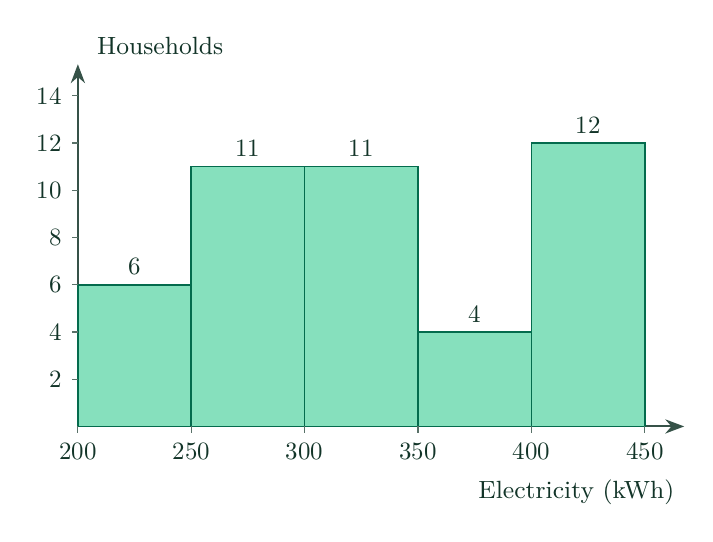
\begin{tikzpicture}
\draw[ink!85, line width=0.7pt, -{Stealth[length=2.4mm]}] (0,0) -- (7.700,0);
\draw[ink!85, line width=0.7pt, -{Stealth[length=2.4mm]}] (0,0) -- (0,4.600);
\draw[draw={rgb,255:red,4;green,107;blue,77}, fill={rgb,255:red,134;green,224;blue,189}, line width=0.6pt] (0.000,0) rectangle (1.440,1.800);
\node[font=\small, text=ink, above] at (0.720,1.800) {$6$};
\draw[draw={rgb,255:red,4;green,107;blue,77}, fill={rgb,255:red,134;green,224;blue,189}, line width=0.6pt] (1.440,0) rectangle (2.880,3.300);
\node[font=\small, text=ink, above] at (2.160,3.300) {$11$};
\draw[draw={rgb,255:red,4;green,107;blue,77}, fill={rgb,255:red,134;green,224;blue,189}, line width=0.6pt] (2.880,0) rectangle (4.320,3.300);
\node[font=\small, text=ink, above] at (3.600,3.300) {$11$};
\draw[draw={rgb,255:red,4;green,107;blue,77}, fill={rgb,255:red,134;green,224;blue,189}, line width=0.6pt] (4.320,0) rectangle (5.760,1.200);
\node[font=\small, text=ink, above] at (5.040,1.200) {$4$};
\draw[draw={rgb,255:red,4;green,107;blue,77}, fill={rgb,255:red,134;green,224;blue,189}, line width=0.6pt] (5.760,0) rectangle (7.200,3.600);
\node[font=\small, text=ink, above] at (6.480,3.600) {$12$};
\draw[ink!70] (0.000,0) -- (0.000,-0.08) node[below, font=\small, text=ink] {$200$};
\draw[ink!70] (1.440,0) -- (1.440,-0.08) node[below, font=\small, text=ink] {$250$};
\draw[ink!70] (2.880,0) -- (2.880,-0.08) node[below, font=\small, text=ink] {$300$};
\draw[ink!70] (4.320,0) -- (4.320,-0.08) node[below, font=\small, text=ink] {$350$};
\draw[ink!70] (5.760,0) -- (5.760,-0.08) node[below, font=\small, text=ink] {$400$};
\draw[ink!70] (7.200,0) -- (7.200,-0.08) node[below, font=\small, text=ink] {$450$};
\draw[ink!70] (0,0.600) -- (-0.08,0.600) node[left, font=\small, text=ink] {$2$};
\draw[ink!70] (0,1.200) -- (-0.08,1.200) node[left, font=\small, text=ink] {$4$};
\draw[ink!70] (0,1.800) -- (-0.08,1.800) node[left, font=\small, text=ink] {$6$};
\draw[ink!70] (0,2.400) -- (-0.08,2.400) node[left, font=\small, text=ink] {$8$};
\draw[ink!70] (0,3.000) -- (-0.08,3.000) node[left, font=\small, text=ink] {$10$};
\draw[ink!70] (0,3.600) -- (-0.08,3.600) node[left, font=\small, text=ink] {$12$};
\draw[ink!70] (0,4.200) -- (-0.08,4.200) node[left, font=\small, text=ink] {$14$};
\node[font=\small, text=ink, anchor=north east] at (7.700,-0.55) {Electricity (kWh)};
\node[font=\small, text=ink, anchor=south west] at (0.12,4.600) {Households};
\end{tikzpicture}
\end{document}
